%%%%%%%%%%%%%%%%%%%%%%%%%%%%%%%%%%%%%%%%%%%%%%%%%%%%%%%%%%%%%%%%%%%%%
% LaTeX Template: Project Titlepage Modified (v 0.1) by rcx
%
% Original Source: http://www.howtotex.com
% Date: February 2014
% 
% This is a title page template which be used for articles & reports.
% 
% This is the modified version of the original Latex template from
% aforementioned website.
% 
%%%%%%%%%%%%%%%%%%%%%%%%%%%%%%%%%%%%%%%%%%%%%%%%%%%%%%%%%%%%%%%%%%%%%%

\documentclass[12pt]{report}
\usepackage[a4paper]{geometry}
\usepackage[myheadings]{fullpage}
\usepackage{fancyhdr}
\usepackage{lastpage}
\usepackage{graphicx, wrapfig, subcaption, setspace, booktabs}
\usepackage[T1]{fontenc}
\usepackage[font=small, labelfont=bf]{caption}
\usepackage{fourier}
\usepackage[protrusion=true, expansion=true]{microtype}
\usepackage[english]{babel}
\usepackage{sectsty}
\usepackage{url, lipsum}
\usepackage{amsmath}


\newcommand{\HRule}[1]{\rule{\linewidth}{#1}}
\onehalfspacing
\setcounter{tocdepth}{5}
\setcounter{secnumdepth}{5}

%-------------------------------------------------------------------------------
% HEADER & FOOTER
%-------------------------------------------------------------------------------
\pagestyle{fancy}
\fancyhf{}
\setlength\headheight{15pt}
\lhead{Egg Drop Vehicle Project}
\fancyhead[R]{Surya Dantuluri}
\fancyfoot[R]{Page \thepage\ of \pageref{LastPage}}
%-------------------------------------------------------------------------------
% TITLE PAGE
%-------------------------------------------------------------------------------

\begin{document}

\title{ \normalsize \textsc{}
		\\ [2.0cm]
		\HRule{0.5pt} \\
		\LARGE \textbf{{Egg Drop Vehicle Project}}
		\HRule{2pt} \\ [0.5cm]
		\normalsize \today \vspace*{5\baselineskip}}

\date{}

\author{
		Surya Dantuluri \\
		Monta Vista High School \\
		AP Physics 1}

\maketitle
\tableofcontents

%-------------------------------------------------------------------------------
% Section title formatting
\sectionfont{\scshape}
%-------------------------------------------------------------------------------

%-------------------------------------------------------------------------------
% BODY
%-------------------------------------------------------------------------------

\chapter{Process}
\section{Design Process}
\qquad Initially my idea was to create a big vehicle that would slowly descend because of drag. This big vehicle would maintain stability by rotating and eventually land on the ground. My initial idea, however, exceeded the weight rule of 100 grams. This was because the combination of a heavy and robust base with a large wing span and large wings were too heavy, even when built with lightweight balsa wood. 

This is why for the second iteration, I designed wings that were as large as the ones I previously built for my initial idea yet were significantly lighter. Instead of using cardboard, I used light balsa wood to be the wings. This second idea still was heavy and I was unsure how rigid the wings were to actually rotate the vehicle. This is because the arms of wings could not be properly mounted to the base of the vehicle.

My third and final reiteration of my vehicle incorporated large wings, a large wingspan and a rigid base. These elements gave stability to the vehicle while maintaining weight. More importantly, the third reiteration distributed weight more evenly by thinning the base of the vehicle to allow for a larger wingspan. This is logical since the base is thick enough for ground impact and the conglomerate vehicle isn't stable enough for its size. Moreover, by removing the top section of the base of the vehicle, the base became even thinner, allowing for more space for the arms to set in place, strenthening the wings, giving the vehicle the capability to rotate more. The wings were also reingineered to be made of aluminum foil with minimal balsa wood scaffholding to keep the wings rigid. Lastly, airflow within the base was considered to be an issue with the design, since the base is very large and is opening downward. To combat this, aluminum foil was placed on all sides of the base, forcing air to go through the vehicle, exiting through the top of the vehicle. This reinforces stability since air that exits through the top is faster, thrusting the vehicle downards.

\section{Testing Design}
All three iterations of the vehicle were tested from a height of 2 meters.\newline 


\hspace*{-0.7cm}\textbf{How I tested my ideas}


I dropped them from my neighbor's apartment, which was on the second story. By testing it from a distance of 2 meters, I could understand what could possibly be an issue when dropping it from a far higher height.

Using this method of testing, I found various flaws with my design, causing me to reiterate over the problems and fixing them in the next design.

For example, when testing I found my intial iteration was unstable and heavy. This was a result of the heavy wings. This method of trial on a small scale and error gave me insight on what to fix and what problems may occur on test day.\newline \newline
\textbf{What I learned from each test}
\begin{itemize}
	\item I learned from the first test that the wings were heavy, causing the vehicle to be unstable, ultimately crashing the vehicle.
 	\item From the second test I learned that the arms for the wings weren't supported enough to rotate the vehicle.
\end{itemize}


From these tests, my final iteration worked better than expected and far better than the previous iterations.


\section{Timeline of Design}
I spent an hour thinking and sketching out possible ideas. I used a notebook to sketch 5-10 different ideas and finally decided on one. 

I spent 2 hours collecting materials. In order to get the wood for my project, I had to travel down to a hobby store relatively far away from me.

I spent 3 hours designing the first prototype since I had to sketch each angle for every truss and glue the foundation together. I spent 5 hours desining and prototyping my 2nd iteration of my vehicle design. This was since I needed to build another base which was lighter and had to make significantly ligher wings. I spent 16 hours on my last iteration since I had to individually sand, chip, and drill the base to make it ligher. Moreover, I had to overhaul the design of the wings and find ligher arms. Moreover, I had to design and manufacture the airflow system in the vehicle, to increase stability. Some of the 16 hours was spent waiting for the Cyanoacrylate fast-drying glue to dry and ventilating my workspace.


\section{Materials Used}
\begin{itemize}
  \item Balsa Wood
  \item Bass Wood
  \item Cyanoacrylate (Glue)
  \item Duct-tape
  \item Aluminum Foil
\end{itemize}







\chapter{Drawings}
\textbf{Note: All Drawings are drawn to scale}
\section{Front Side of Vechicle}
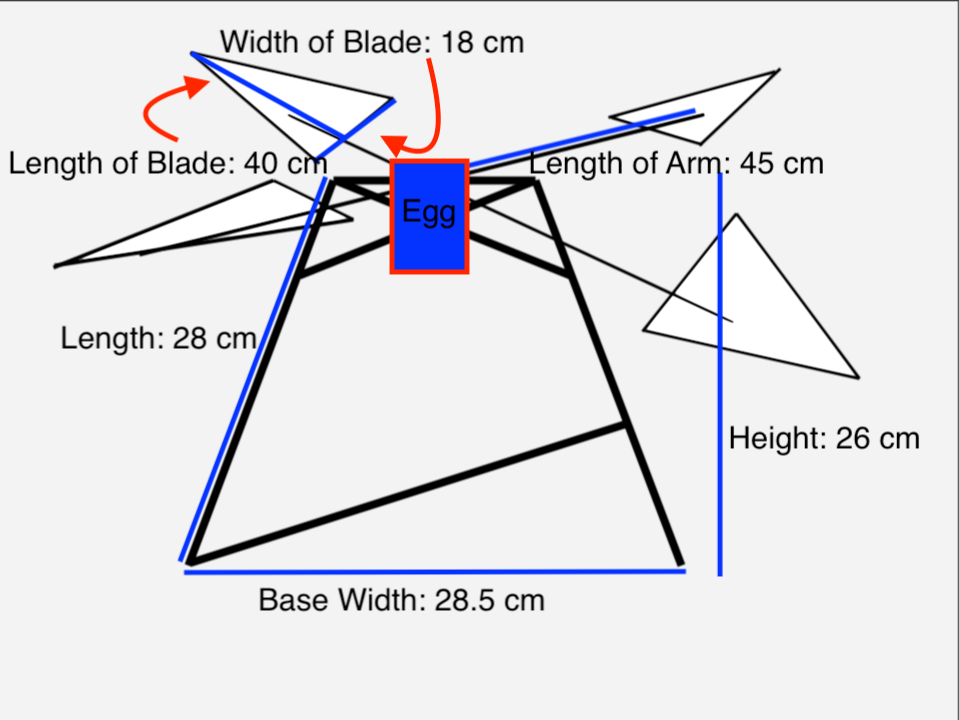
\includegraphics[width=15cm, height=8cm]{egg_final}
\section{Sides of Vehicle}
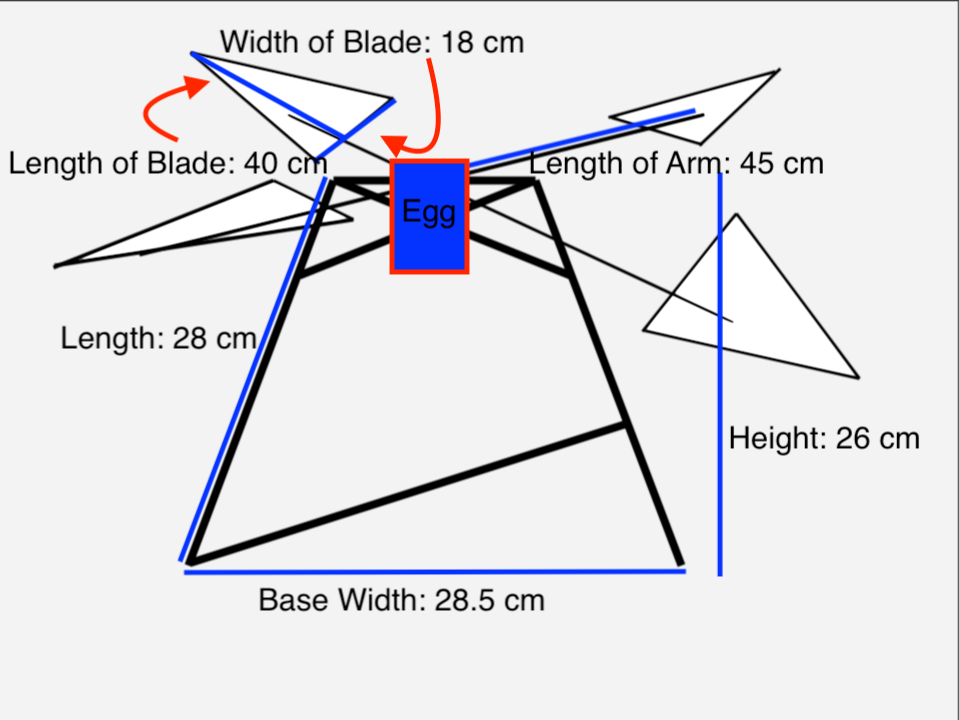
\includegraphics[width=15cm, height=8cm]{egg_final}
\section{Top of Vehicle}
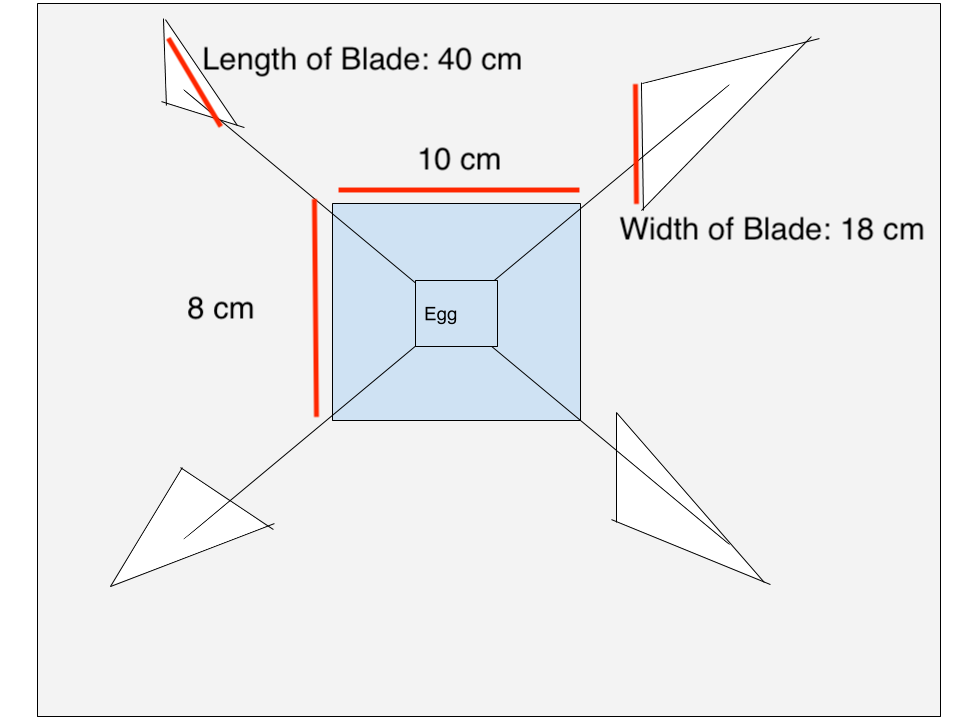
\includegraphics[width=15cm, height=8cm]{top_egg}

\chapter{Photograph}
\section{Front Side of Vechicle}
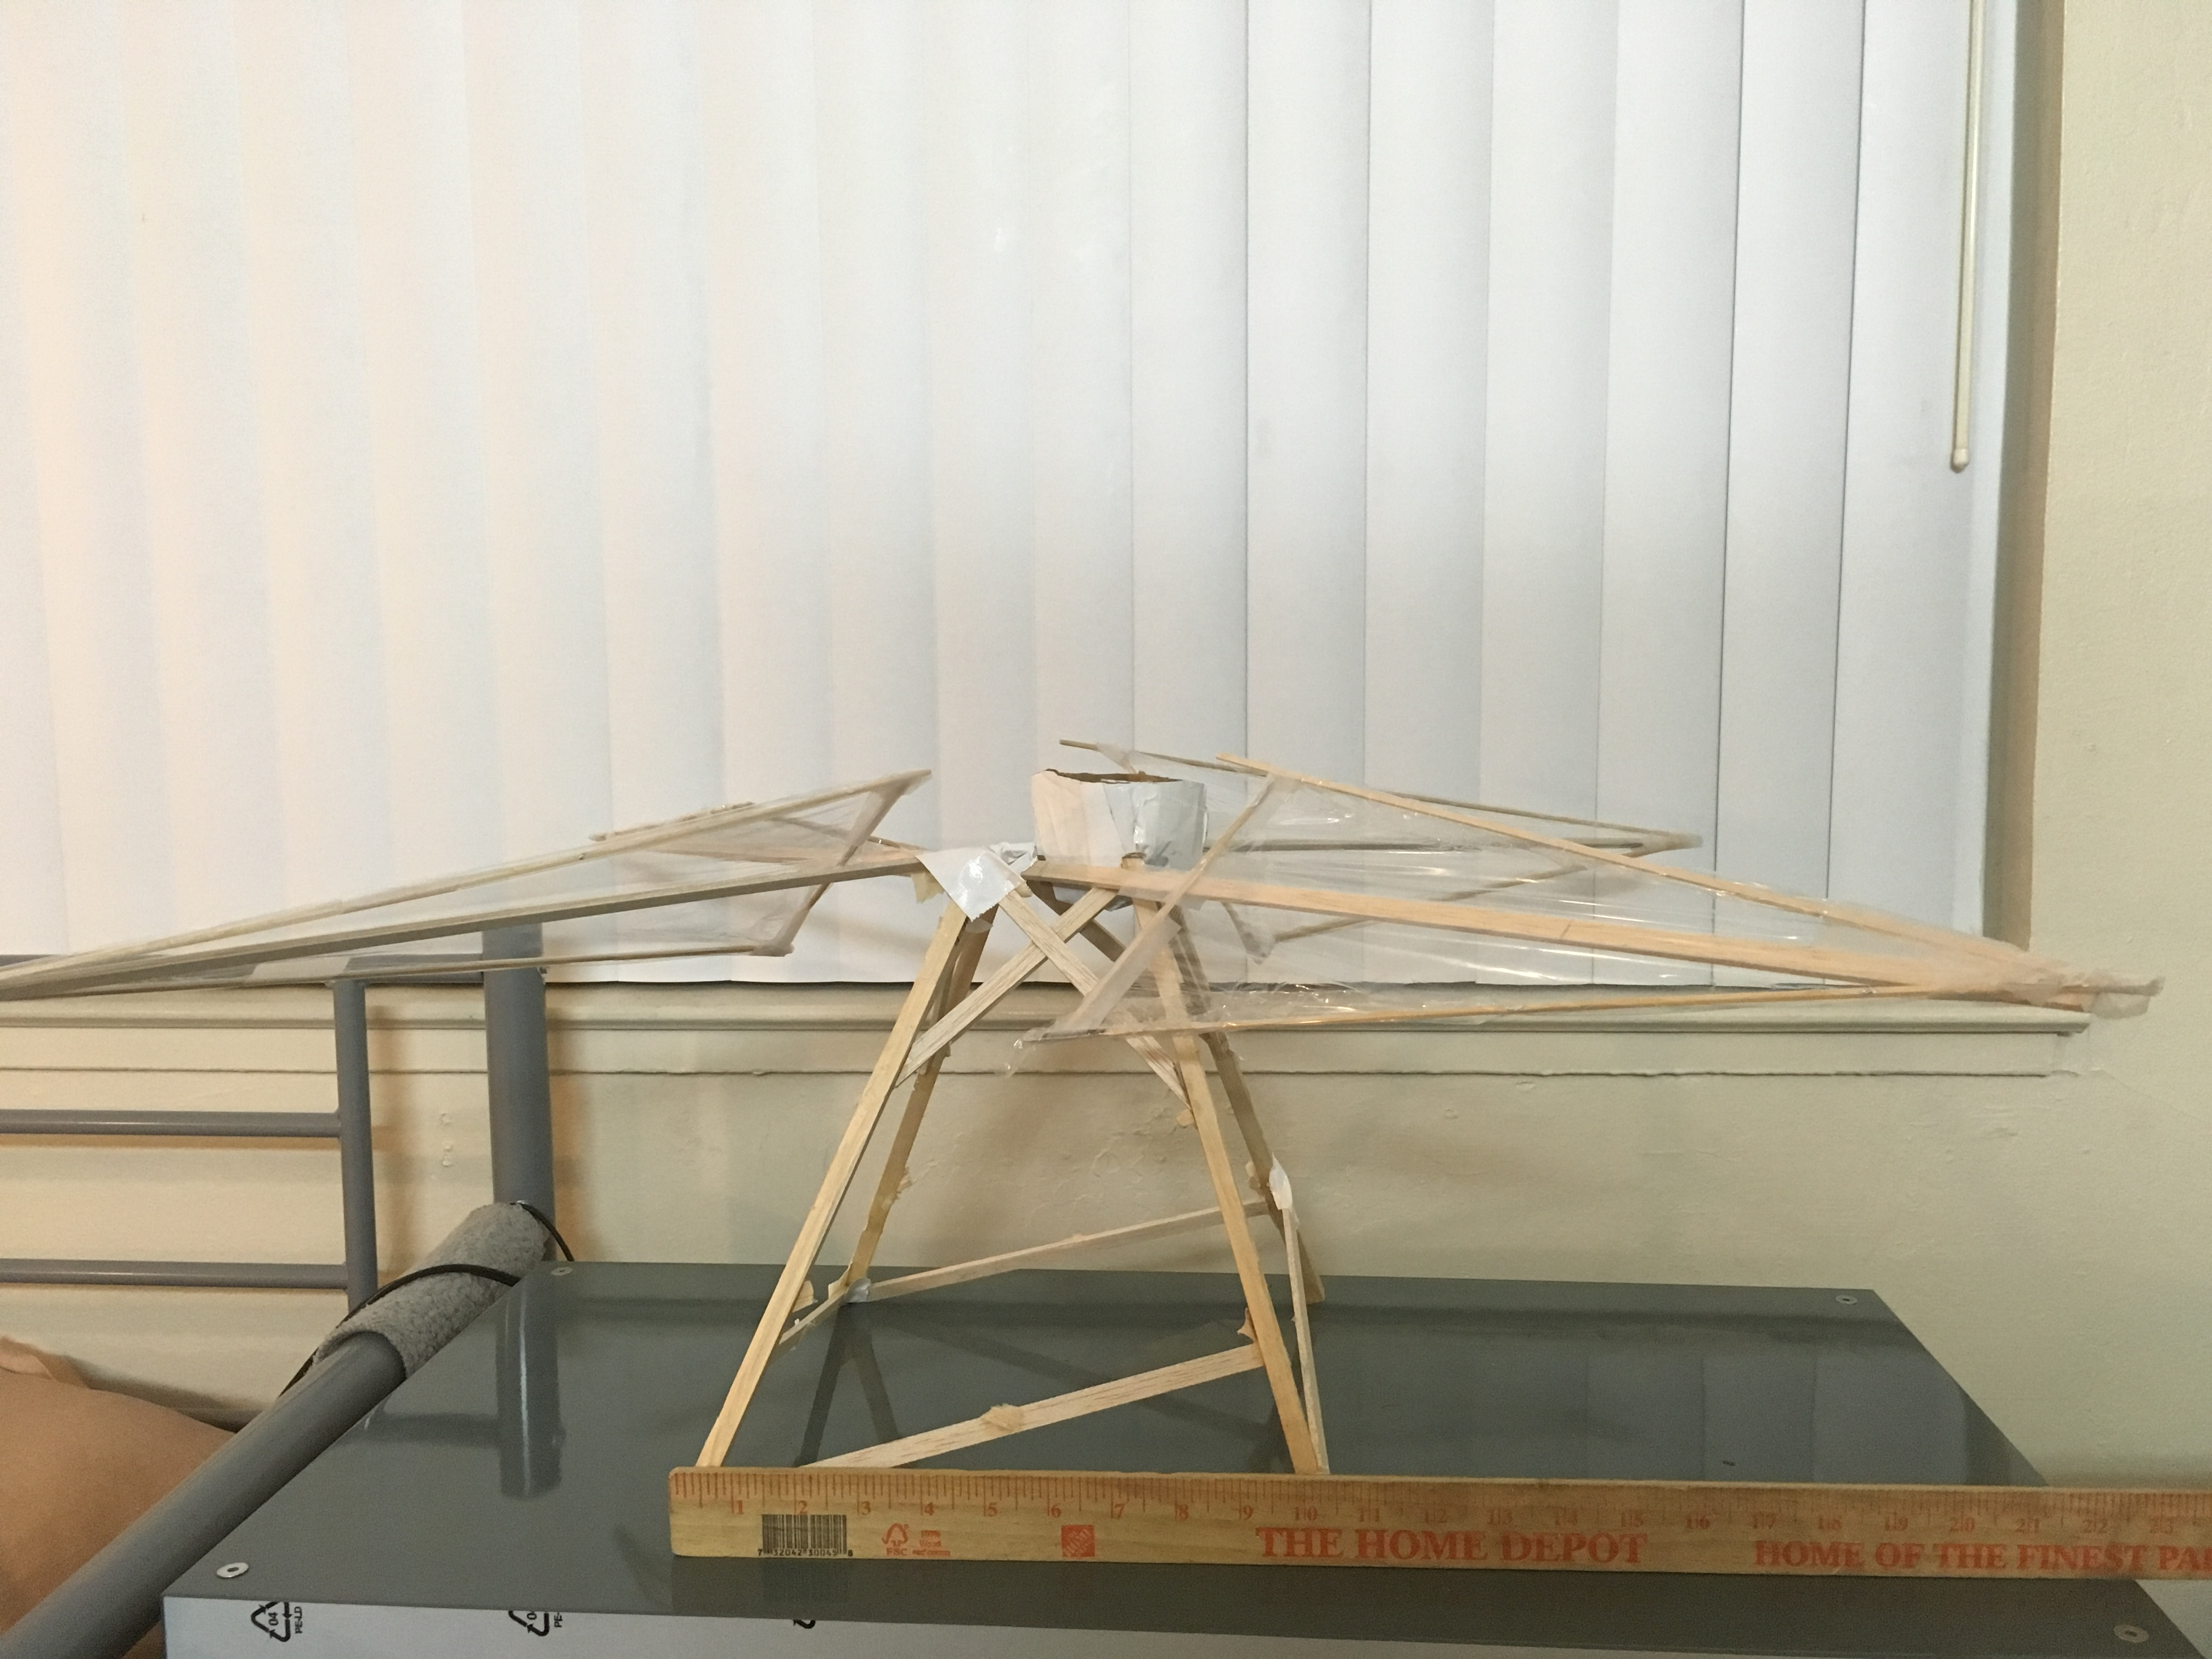
\includegraphics[width=15cm, height=8cm]{front}
\section{Sides of Vehicle}
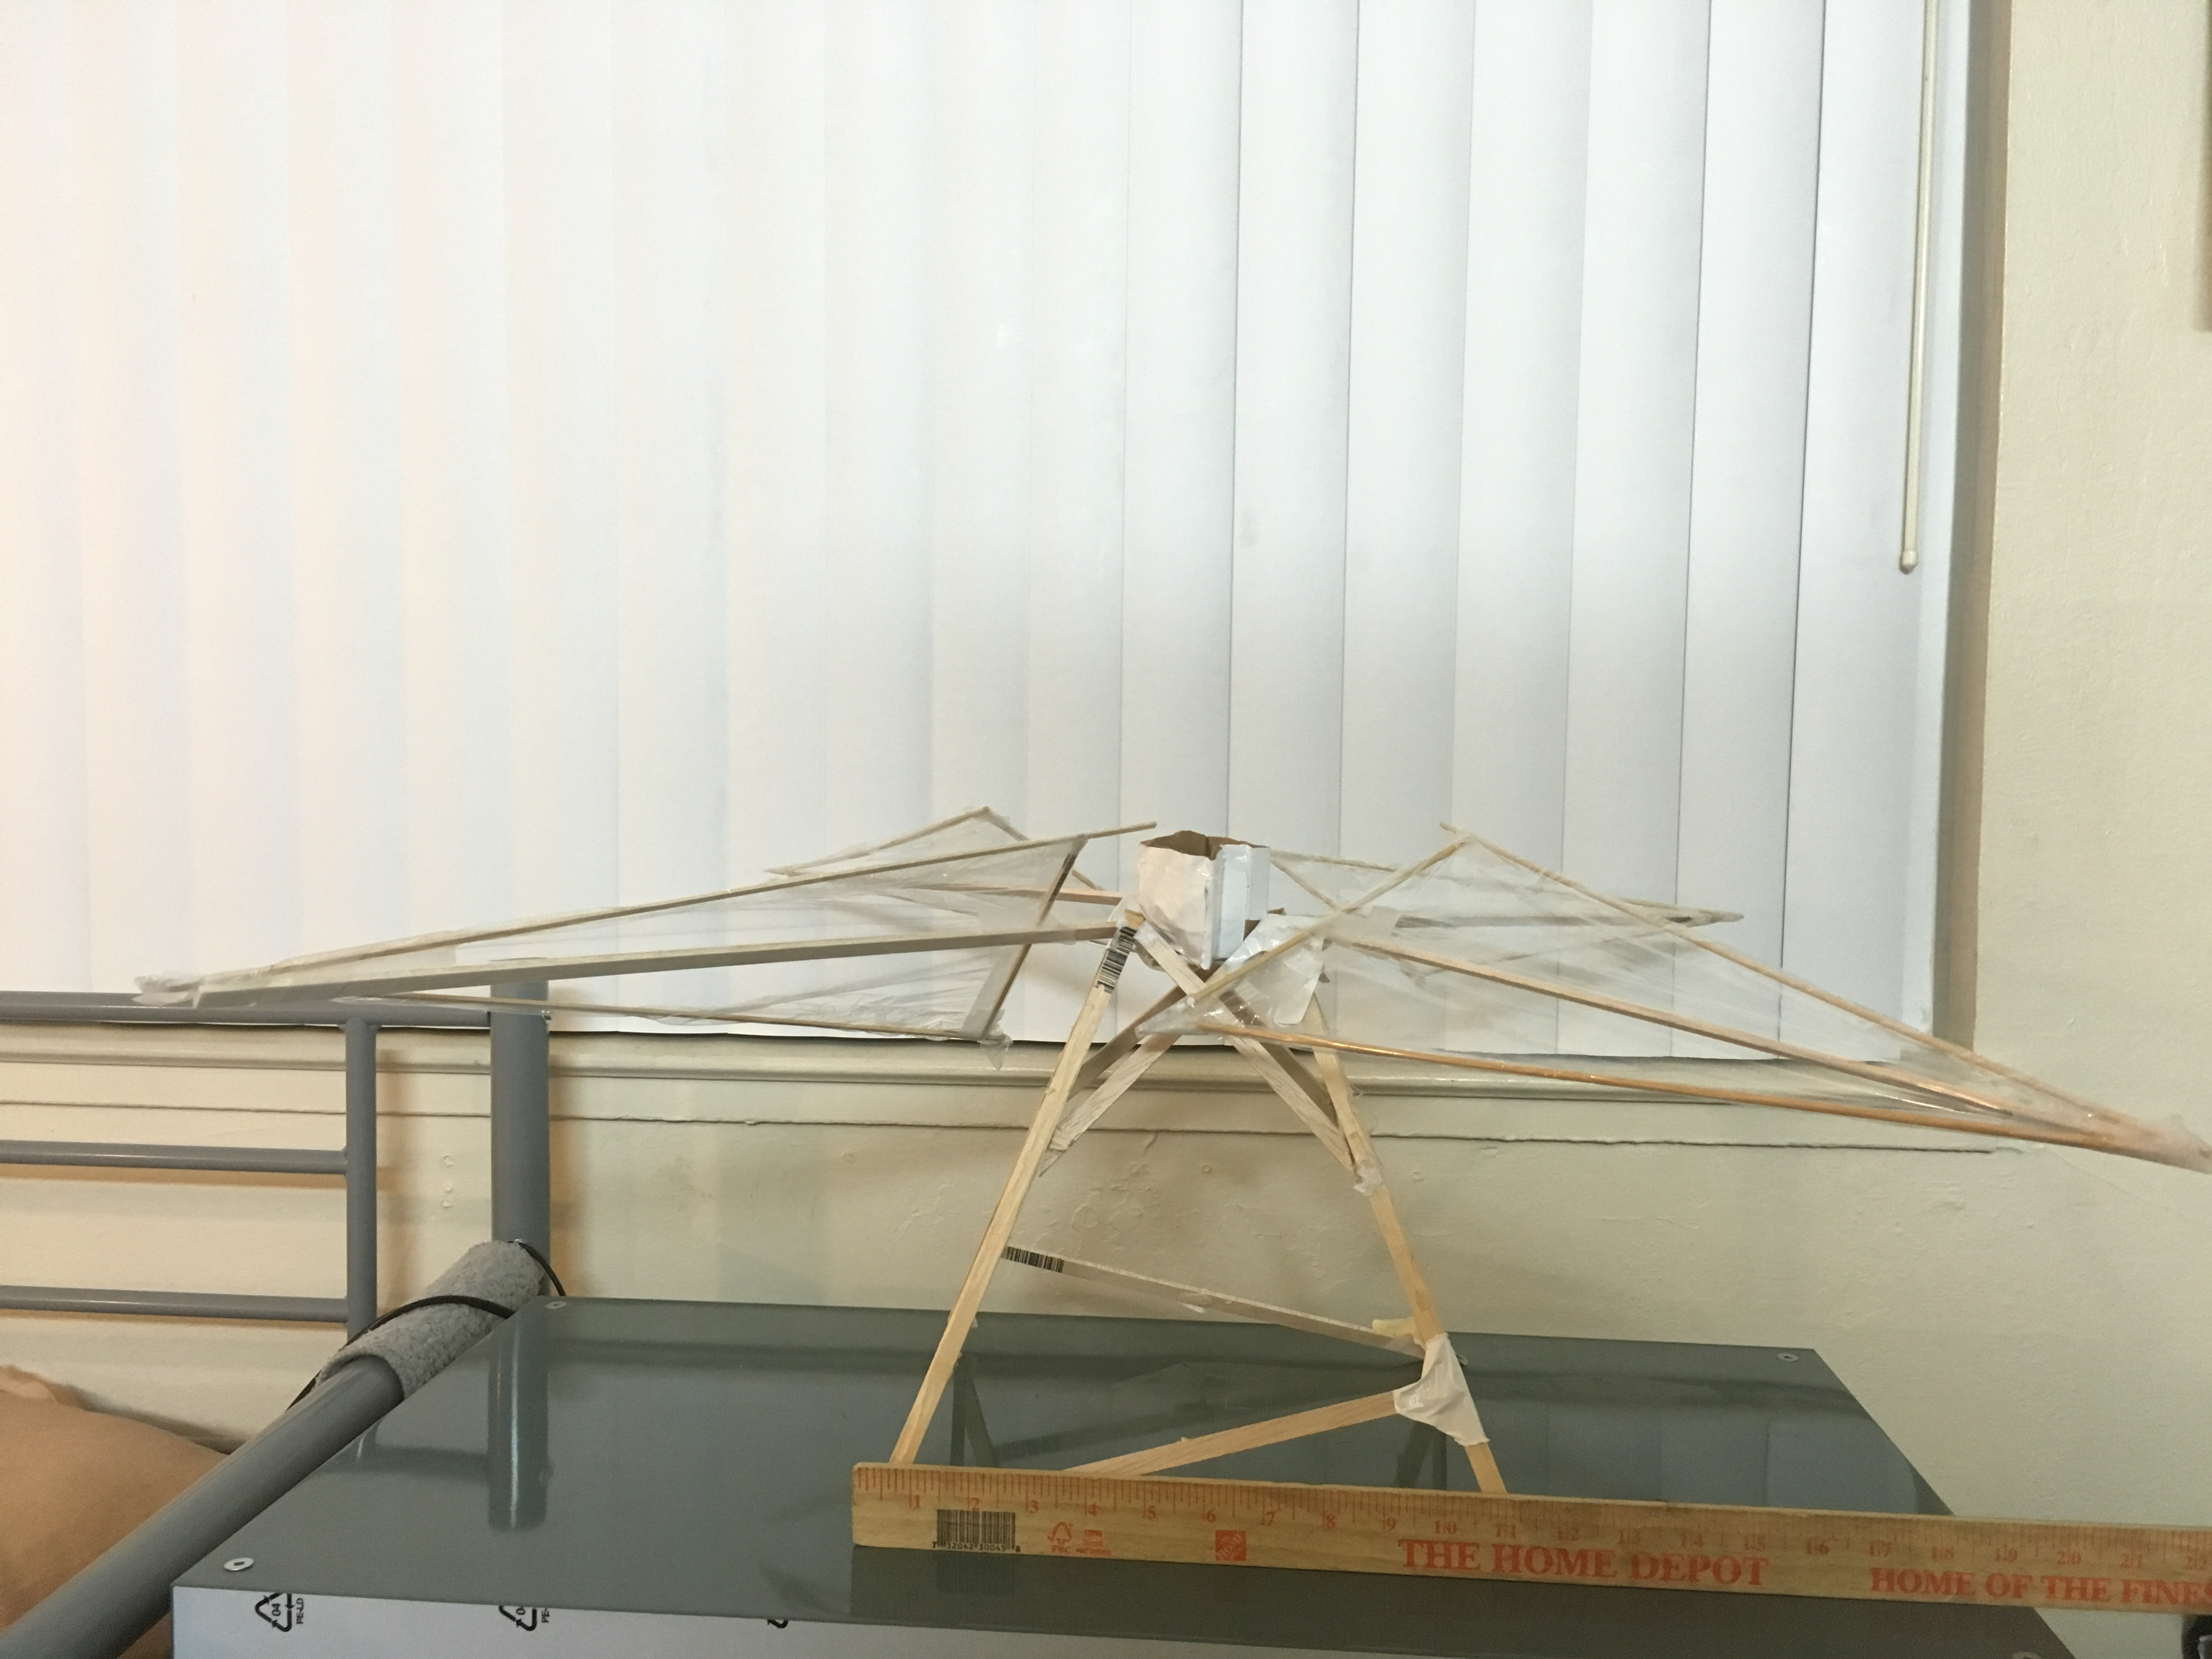
\includegraphics[width=15cm, height=8cm]{side}
\newline \newline
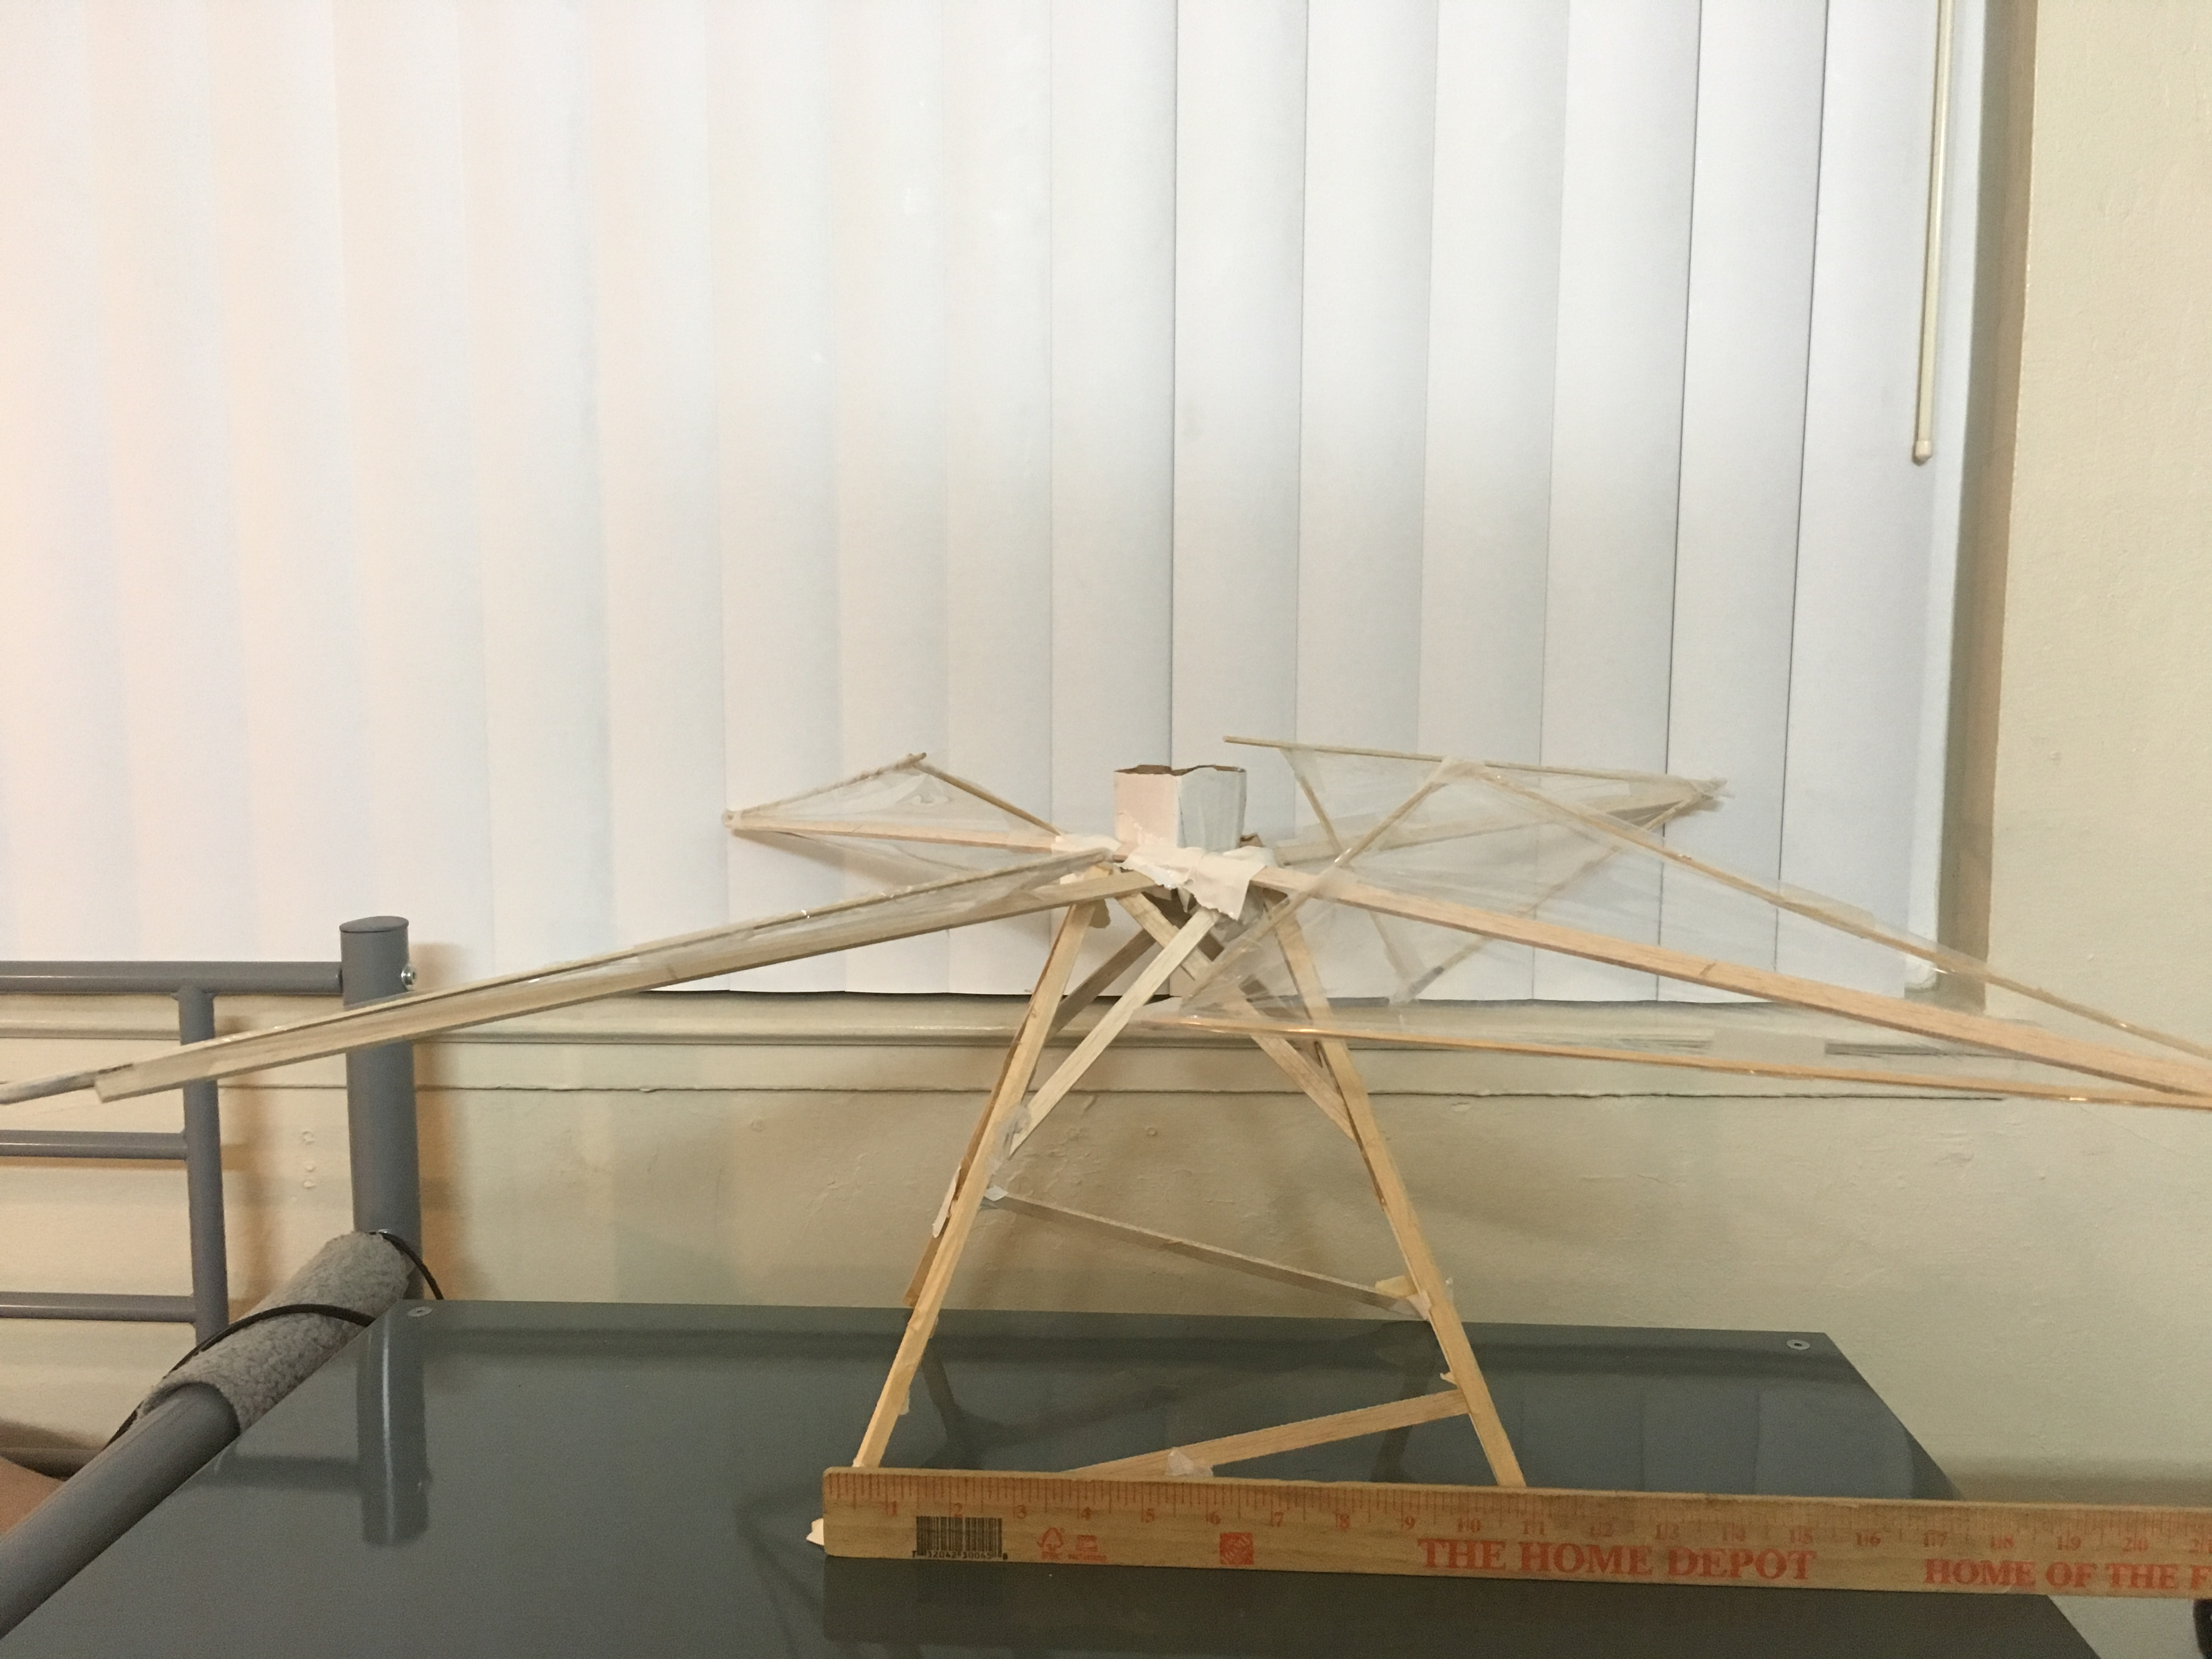
\includegraphics[width=15cm, height=8cm]{side2}
\section{Top of Vehicle}
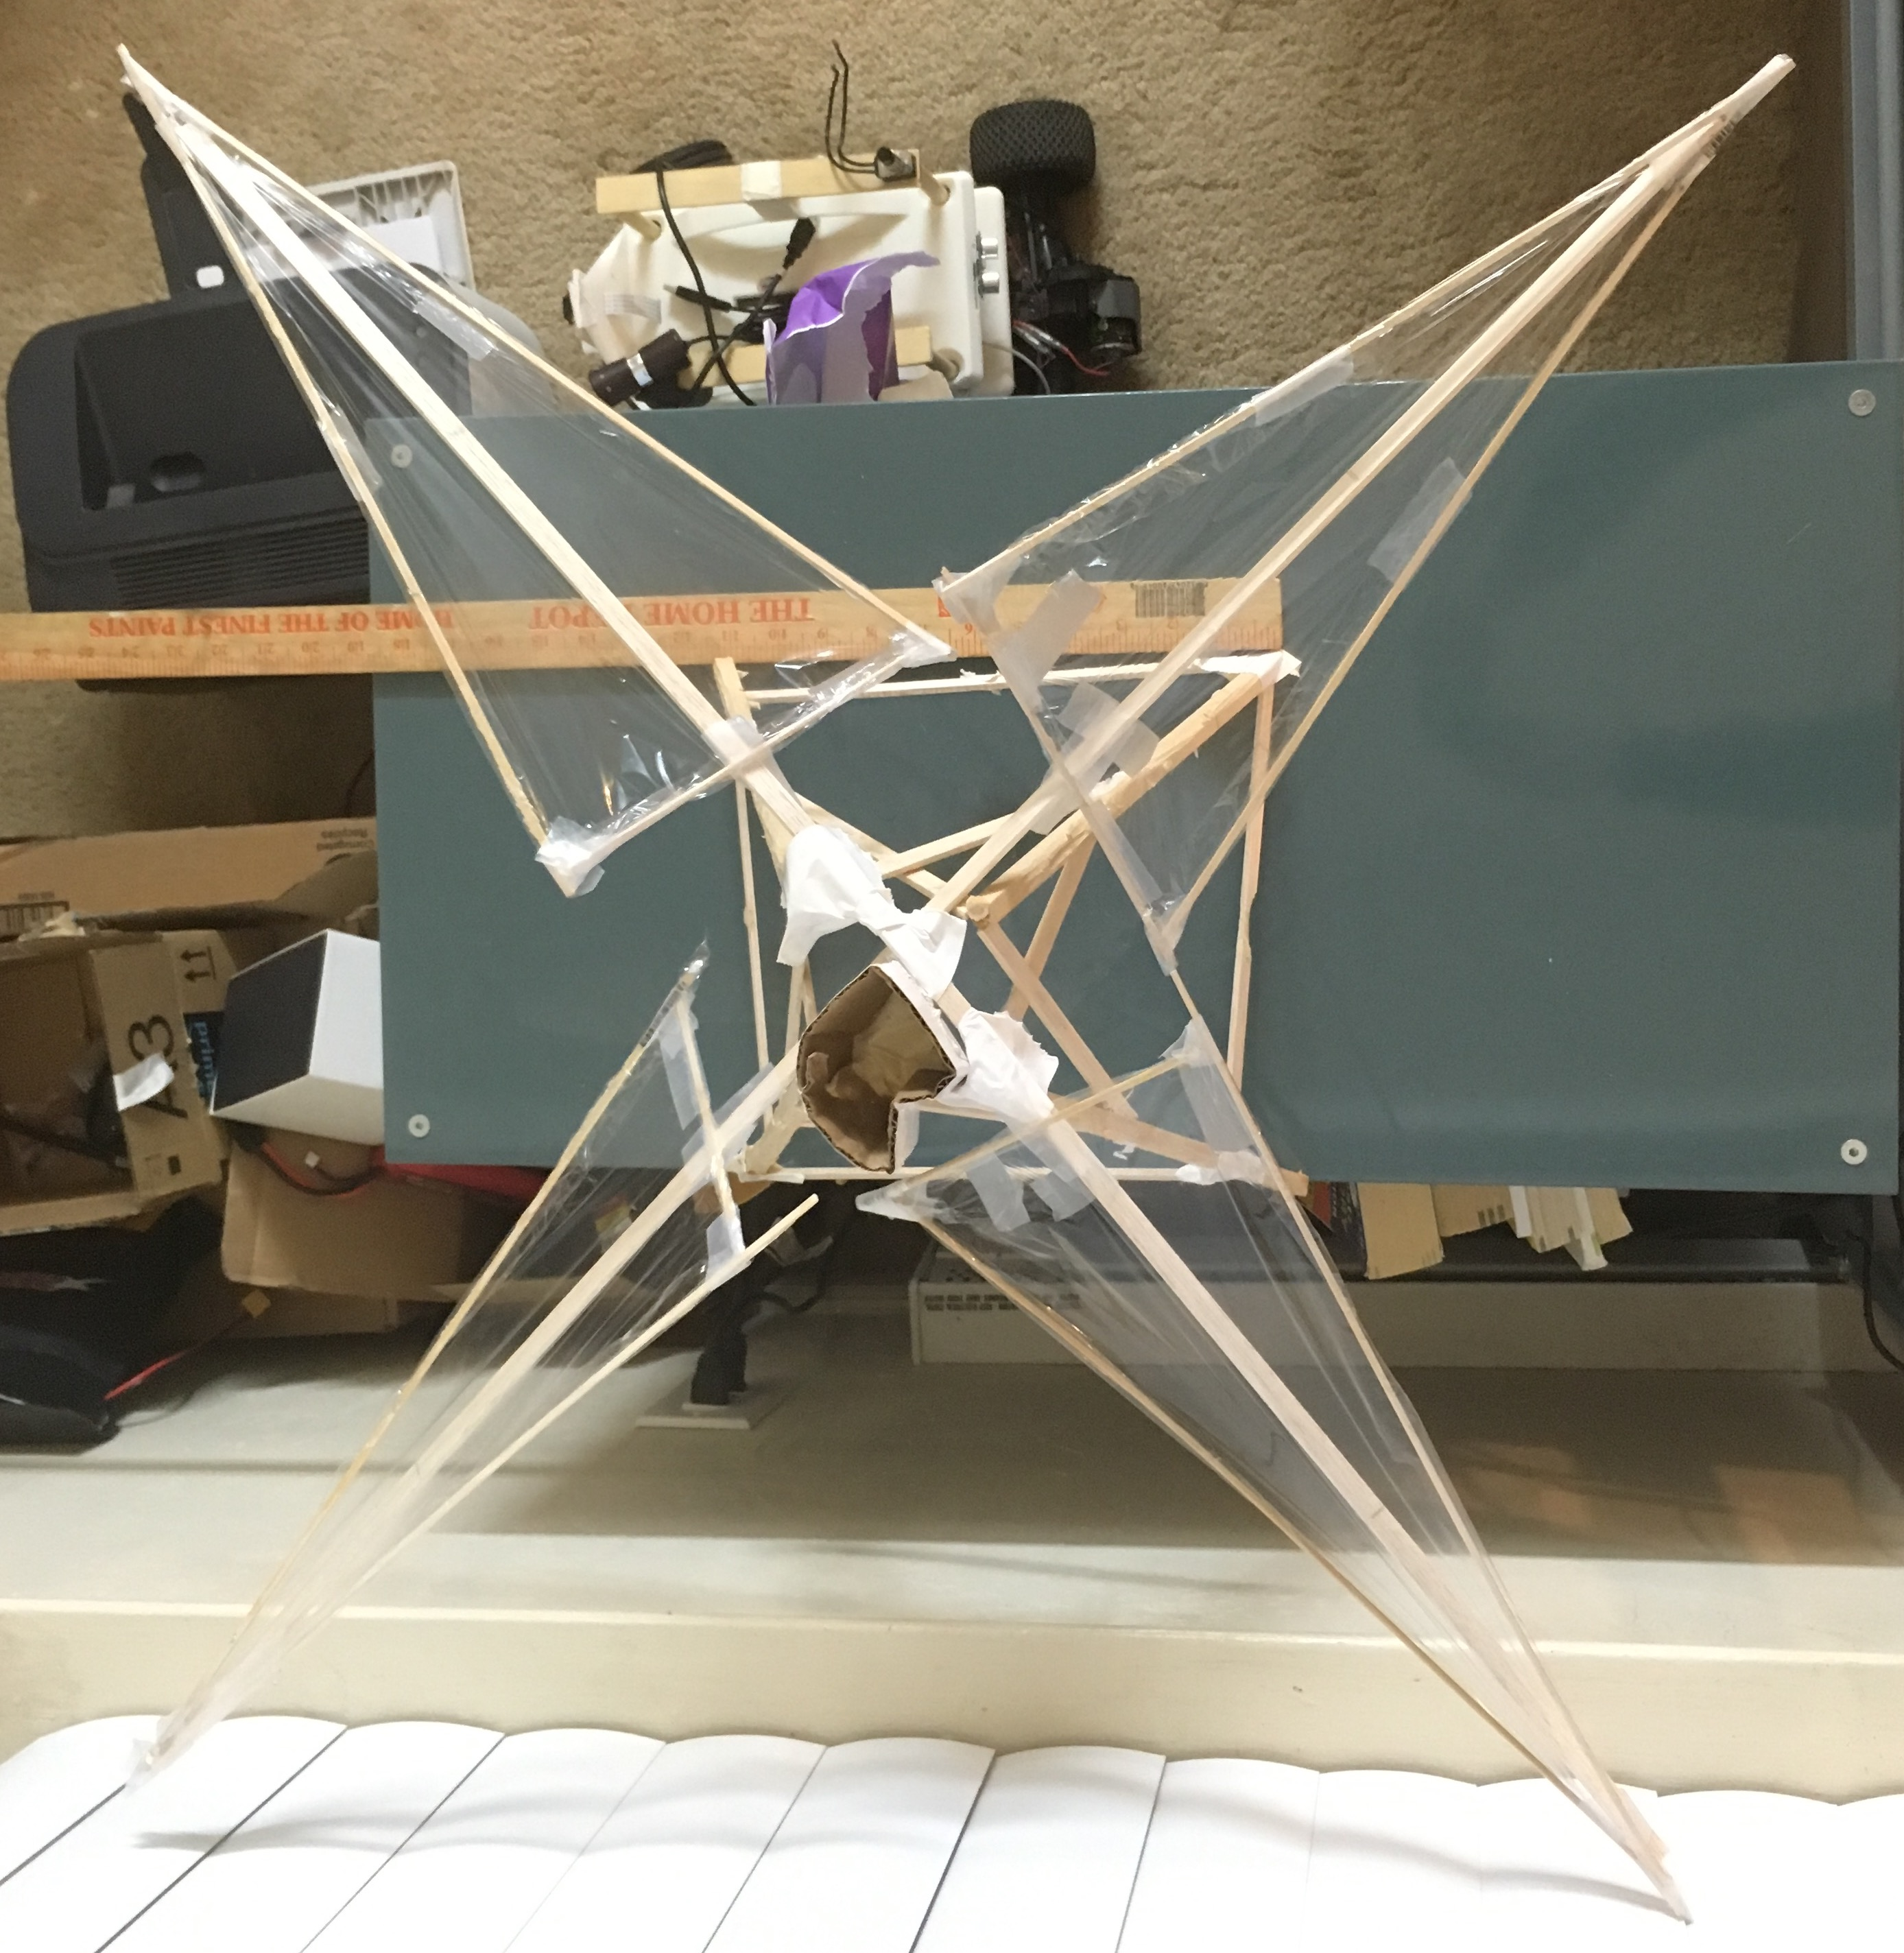
\includegraphics[width=15cm, height=8cm]{top}


\chapter{Controlling Vehicle Speed and Rotation}



\section{Speed Control: Linear Dynamics}

\qquad According to Newton's 2nd law of motion, $F_{net} = ma$ where $F$ is force and $m$ is mass and $a$ is acceleration. In this situation, as the vehicle is dropped from a height $h$, air resistance, $ F_{air} $ counteracts the gravitational force, $ F_{g} $. This would mean the net force of the vehicle would be $F_{g} - F_{air}$
Applying Newton's 2nd law, we can deduce
\begin{equation} \label{eq:1}
F_{g} - F_{air} = ma
\end{equation}
 in this situation. From equation \ref{eq:1} we can find $F_{air}$ is directly proportional to negative acceleration, $-a$ since we can't control gravitational force (since it is constant throughout the drop) and mass $m$ is a constant too.
 Since $F_{air}$ is directly proportional to negative acceleration, $-a$, I tried to maximize air resistance as much as possible. This would minimize acceleration and result in a slow descend of the vehicle downward, which is ideal to keep the egg intact. I decided to use large wings to maximize this air resistance force and shape the base of my vehicle in a cone shape to increase air contact, increasing the air resistance force.
% like\textsubscript{this}

%Use kinematics equations to explain how you kept the vehicle from striking the ground at high speed.
\section{Speed Control: Linear Kinematics}
The goal here is to reduce the final velocity, $v_f$ of the vehicle when it hits the ground. To understand how I could accomplish this, I used the kinematics equation $v_f^2 = v_i^2 + 2a\Delta x$ where $a$ is acceleration and $x$ is distance in meters. In this instance, $x$ should be height $h$ from the height of the drop to the ground, making the equation 
\begin{equation} \label{eq:2}
v_f^2 = v_i^2 + 2a\Delta h
\end{equation}. When the vehicle is dropped from rest, $v_i$ is 0 and $\Delta h$ is a constant. This is because the vehicle initially has no velocity and the distance from where it is dropped is constant. This means the equation can be simplified to 
\begin{equation} \label{eq:3}
v_f^2 = 2a\Delta h
\end{equation} 
.  This means $2a\Delta h$ is the constant of proportionality and $v_f^2$ is directly proportional to acceleration $a$.
Since $v_f^2$ is directly proportional to acceleration $a$ and we want to reduce the final velocity, I need to find a way to decrease acceleration.\newline \newline
As explained in the previous section, I used large wings and a cone structure to increase air contact, increasing air resistance, resulting in a decrease in acceleration. Since the acceleration decreases and the final velocity is directly proportional to the acceleration, the final velocity of the egg and the vehicle will be lower, effectively reaching the goal of reducing the final velocity.

\section{Rotation Control: Angular Dynamics}
Rotation played an important role in maintaining stability. The blades of the vehicle are tilted at a certain angle, so when the vehicle is descending, they exert a normal force on the air.  The normal force $F_n$ is has both a vertical and horizontal componnets, where the vertical component of $F_n$ is the drag created by the blades, while the horizontal component is $ F_n*cos(\theta)$, where $\theta$ is the tilt of the blades. This horizontal component generates torque, defined as $\tau = r * F$, where r is the vector from the center of the blade to the axis of rotation, which is the center of the vehicle. F is horizontal component perpendicular to r, which is $ F_n*cos(\theta)$. This means the torque of one blade on the vehicle can be represented as $\tau = r * F_n*cos(\theta)$. This torque causes the vehicle to spin, represented as $\tau = I*\omega$. $I$ is the moment of intertia of the vehicle and $\omega$ is the angular velocity. Moreover, Since the net torque is not zero (because of the blades), the vehicle's angular acceleation cannot be zero either, meaning the torque acting on the vehicle is proportional to the angular acceleration, which causes the vehicle to rotate. Since $KE = (1/2)*I*\omega^2$ and in this scenario $KE_f = \Delta PE + W_{nc}$ where $KE$ includes both linear and rotational, an increase in rotational $KE$ causes a lower linear $KE$ since $\Delta PE + W_{nc}$ is constant. This means the vehicle will descend slower with more rotational $KE$, which is ideal to preven the egg from cracking.



\section{Rotation Control: Energy Conservation}
The conservation of energy equation is as follows: 
\begin{equation} \label{eq:4}
W_{nc}+K_0+U_{eo}+U_{go} = K_{f}+U_{ef}+U_{gf}
\end{equation}
. In this equation, the nonconservative work with the initial kinetic, spring, and gravitational potential energy is equal to the final kinetic, spring, and gravitational potential energy. In this situation, there is no initial kinetic or spring potential energy. Neither is there final gravitational potential energy since the vehicle will be on the ground with height 0 after falling to the ground or have a final spring potential energy. As a result, our equation turns to be as follows:
\begin{equation} \label{eq:5}
W_{nc}+U_{go} = K_{f}
\end{equation}
This can also be written as follows:

%\begin{align*} \label{eq:6}
%W_{nc}+mgh = 1/2*m*v^2 \\
%W_{nc}+gh = 1/2*m*v^2
%\end{align*}
\begin{equation} \label{eq:6}
W_{nc}+mgh = 1/2*m*v^2
\end{equation}

Since the gravitational potential force and $mgh$ and aa both constants, the nonconservative work is proportional to the final kinetic energy. Since we don't want there to be a high amount of kinetic energy when the vehicle reaches the ground, we'll need to find what kinetic energy is proportional to to figure out what to try to decrease. $KE_f$ is proportional to $W_{nc}$ according to equation \ref{eq:6}. In order to decrease the nonconservative work, I used large airplane wings and a cone design to maximize air resistance or drag by having as much surface area of the vehicle to be creating drag. This drag decreases the nonconservative work done by $F_{air}*d$. Since $W_{nc}$ is directly proportional to $v_f^2$, decreasing nonconservative work decreases the final velocity, leading to a slow landing, which is ideal to prevent the egg from breaking.



\chapter{Maintaining Vehicle Stability}
\section{Statics: Forces and Torques}
The vehicle was kept stable by distributing forces among the blades of the vehicle. Using Newton's 2nd law of rotation, $\tau = I*\alpha$ we can determine how the distribution of forces acts on the vehicle. As shown in the diagram, each blade has a net force of $m_{blade}*g - F_{drag}$. Since the forces of the blades are the same because they are constructed to be the same, their torques are same as well. Since the torques act in opposite direction, the net torque is equal to zero. This means for any constant moment of inertia, the angular acceleration will be zero. This results in stability for the vehicle since the angular acceleration will be zero, in the direction that is perpendicular to the ground.

The vehicle will tip over in the event the drag is greater on one side of the vehicle than the other. This is because the torque, represented as $\tau = F_r$ will be different on each of the blades, depending on the cirumstance. This difference in torque will cause the vehicle to tip over, leading to the failure of the vehicle. To combat this, I designed sturdy blades, which will exert a greater normal force in the event the torques among the blades are different. This greater normal force will self-correct the vehicle and maintain stability.


\chapter{Controlling Impact with the Ground}

\section{Impact: Linear Dynamics}
As the vehicle hit the ground, there are several forces affecting its impact. There is the normal force, $F_n$, gravity, $F_g$, and drag, $F_{drag}$. This means the net force on the egg in the air can be represented by $m*g-F_{drag} = m*a$ since $F_{net} = ma$, according to Newton's 2nd law. Upon impact, however, net force on the egg can be represented as $F_n - F_g = m*a$ according to Newton's 2nd law. This means a lower acceleration or lower mass will reduce the normal force and gravitational force. To do this, I increased drag by designing relatively large wings. This decreases the net force on the egg, which is ideal to prevent the egg from breaking. I also constructed a lightweight structure under a 100 grams, which also reduces net force on the egg.

\section{Impact: Linear Momentum, Impulse, and Collisions}
Ideally, an inelastic collision would be ideal. An inelastic collision would minimize total kinetic energy since it will not be conserved. An inelastic collision would "stick" the vehicle to the ground since the vehicle has come to a complete stop upon impacting the ground. An inelastic collision is also ideal since the egg would not fall out and break as with an elastic collision. However, an ideal inelastic collision is not feasible because of various factors including external forces.

When the egg hits the ground, an impulse on the egg occurs. This impulse is a change in momentum and can be represented as $I = F*t$. Since I is constant, in order to minimize the force on the egg, the time over which the force lasts on the egg must be extended. 

A different way the force on the egg is minimized upon impact is by reducing the mass of the vehicle. Since impulse can also be written as $m\Delta v = Ft$, minimizing the mass of the vehicle reduces the force on the vehicle, which in turn reduces the velocity from what was previously discussed. This leads to a slow and gradual descent of the vehicle, preventing the egg from breaking.

\section{Impact: Work}
The equation for work can be represented as $W = F*d*cos(\theta)$. Since final kinetic energy, $KE_f$ should be zero by the time of impact, $W = \Delta KE = KE_{f}-KE_{initial}$ is equivalent to $W = -KE_{initial}$. From our previous equation, we can substitue to finaly get

\begin{equation} \label{eq:7}
F*d*cos(\theta) = -KE_{initial}
\end{equation}

To decrease forces acted upon the egg, the distance the force acts on the egg needs to be extended. In response to this issue, I made my structure high. This allows the lower body of my structure to be compressed, allowing the forces acting upon the egg to extend.

%
% \chapter{Additional Benefits of Rotation}



\end{document}

%-------------------------------------------------------------------------------
% SNIPPETS
%-------------------------------------------------------------------------------

%\begin{figure}[!ht]
%	\centering
%	\includegraphics[width=0.8\textwidth]{file_name}
%	\caption{}
%	\centering
%	\label{label:file_name}
%\end{figure}

%\begin{figure}[!ht]
%	\centering
%	\includegraphics[width=0.8\textwidth]{graph}
%	\caption{Blood pressure ranges and associated level of hypertension (American Heart Association, 2013).}
%	\centering
%	\label{label:graph}
%\end{figure}

%\begin{wrapfigure}{r}{0.30\textwidth}
%	\vspace{-40pt}
%	\begin{center}
%		\includegraphics[width=0.29\textwidth]{file_name}
%	\end{center}
%	\vspace{-20pt}
%	\caption{}
%	\label{label:file_name}
%\end{wrapfigure}

%\begin{wrapfigure}{r}{0.45\textwidth}
%	\begin{center}
%		\includegraphics[width=0.29\textwidth]{manometer}
%	\end{center}
%	\caption{Aneroid sphygmomanometer with stethoscope (Medicalexpo, 2012).}
%	\label{label:manometer}
%\end{wrapfigure}

%\begin{table}[!ht]\footnotesize
%	\centering
%	\begin{tabular}{cccccc}
%	\toprule
%	\multicolumn{2}{c} {Pearson's correlation test} & \multicolumn{4}{c} {Independent t-test} \\
%	\midrule	
%	\multicolumn{2}{c} {Gender} & \multicolumn{2}{c} {Activity level} & \multicolumn{2}{c} {Gender} \\
%	\midrule
%	Males & Females & 1st level & 6th level & Males & Females \\
%	\midrule
%	\multicolumn{2}{c} {BMI vs. SP} & \multicolumn{2}{c} {Systolic pressure} & \multicolumn{2}{c} {Systolic Pressure} \\
%	\multicolumn{2}{c} {BMI vs. DP} & \multicolumn{2}{c} {Diastolic pressure} & \multicolumn{2}{c} {Diastolic pressure} \\
%	\multicolumn{2}{c} {BMI vs. MAP} & \multicolumn{2}{c} {MAP} & \multicolumn{2}{c} {MAP} \\
%	\multicolumn{2}{c} {W:H ratio vs. SP} & \multicolumn{2}{c} {BMI} & \multicolumn{2}{c} {BMI} \\
%	\multicolumn{2}{c} {W:H ratio vs. DP} & \multicolumn{2}{c} {W:H ratio} & \multicolumn{2}{c} {W:H ratio} \\
%	\multicolumn{2}{c} {W:H ratio vs. MAP} & \multicolumn{2}{c} {\% Body fat} & \multicolumn{2}{c} {\% Body fat} \\
%	\multicolumn{2}{c} {} & \multicolumn{2}{c} {Height} & \multicolumn{2}{c} {Height} \\
%	\multicolumn{2}{c} {} & \multicolumn{2}{c} {Weight} & \multicolumn{2}{c} {Weight} \\
%	\multicolumn{2}{c} {} & \multicolumn{2}{c} {Heart rate} & \multicolumn{2}{c} {Heart rate} \\
%	\bottomrule
%	\end{tabular}
%	\caption{Parameters that were analysed and related statistical test performed for current study. BMI - body mass index; SP - systolic pressure; DP - diastolic pressure; MAP - mean arterial pressure; W:H ratio - waist to hip ratio.}
%	\label{label:tests}
%\end{table}